\documentclass[conference]{IEEEtran}
\IEEEoverridecommandlockouts

\usepackage{cite}
\usepackage{amsmath,amssymb,amsfonts}
\usepackage{graphicx}
\usepackage{textcomp}
\usepackage{xcolor}

\usepackage{subcaption}

\usepackage{tikz}
\usepackage{pgfplots}

\usepackage{cleveref}
\usepackage{csquotes}
\usepackage{booktabs}

\usepackage{flushend}


\definecolor{tol1}{HTML}{33bbee}
\definecolor{tol2}{HTML}{009988}
\definecolor{tol3}{HTML}{ee7733}
\definecolor{tol4}{HTML}{cc3311}

\usepackage{acro}
\DeclareAcronym{cots}{
  short = COTS,
  long = off-the-shelf,
}

\DeclareAcronym{tiff}{
  short = TIFF,
  long = tag image file format,
}

\DeclareAcronym{mse}{
  short = MSE,
  long = mean squared error,
}

\DeclareAcronym{awgn}{
  short = AWGN,
  long = additive white Gaussian noise,
}

\DeclareAcronym{leo}{
  short = LEO,
  long = low Earth orbit,
}

\DeclareAcronym{ldpc}{
  short = LDPC,
  long = low-density parity-check,
}

\DeclareAcronym{jscc}{
  short = JSCC,
  long = joint source and channel coding,
}

\DeclareAcronym{djscc}{
  short = DJSCC,
  long = deep joint source and channel coding,
}

\DeclareAcronym{snr}{
  short = SNR,
  long = signal-to-noise ratio,
}

\DeclareAcronym{cnn}{
  short = CNN,
  long = convolutional neural network,
}

\DeclareAcronym{psnr}{
  short = PSNR,
  long = peak signal-to-noise ratio,
}

\DeclareAcronym{prelu}{
  short = PReLU,
  long = parameterized rectified linear unit,
}

\DeclareAcronym{jscc-sat}{
  short = \textsc{JSCC-Sat},
  long = {joint source-and-channel coding for small satellite applications}
}

\DeclareAcronym{los}{
  short = {LOS},
  long = {line of sight}
}

\DeclareAcronym{esa}{
  short=ESA,
  long=European Space Agency
}

\usepackage{xspace}
\newcommand\cubesat{CubeSat\xspace}
\newcommand\cubesats{\cubesat{}s\xspace}

\newcommand\jpegtwok{JPEG\,2000\xspace}

\newcommand\sentinelii{Sentinel-2\xspace}

\begin{document}

\title{Adaptable Joint Source-and-Channel Coding for Small Satellite Applications}

\author{\emph{Anonymous authors}}
% \author{\IEEEauthorblockN{Olga Kondrateva}
% \IEEEauthorblockA{\textit{Humboldt-Universit\"at zu Berlin}\\
% Berlin, Germany \\
% kondrate@informatik.hu-berlin.de}
% \and
% \IEEEauthorblockN{Stefan Dietzel}
% \IEEEauthorblockA{\textit{Merantix Momentum GmbH}\\
% Berlin, Germany \\
% stefan@merantix-momentum.com}
% \and
% \IEEEauthorblockN{Bj\"orn Scheuermann}
% \IEEEauthorblockA{\textit{Technical University of Darmstadt}\\
% Darmstadt, Germany \\
% scheuermann@kom.tu-darmstadt.de}
% }

\maketitle

\begin{abstract}
Earth observation using small satellites serves a wide range of relevant applications.
However, significant advances in sensor technology (e.g., higher resolution, multiple spectrums beyond visible light) in combination with challenging channel characteristics lead to a communication bottleneck 
when transmitting the collected data to Earth.
Recently, joint source coding, channel coding, and modulation using a neuronal-network-based approach has been proposed to combine image compression and communication. %dynamically adapt to the varying communication channel and to take data properties into account.
Though this approach achieves promising results when applied to standard terrestrial channel models, 
it remains an open question whether it is suitable for the more complicated and quickly varying satellite communication channel. 
In this paper, we consider a detailed satellite channel model accounting for different shadowing conditions and train an encoder-decoder architecture using realistic \sentinelii satellite imagery.
In addition, to reduce the overhead associated with using multiple neural networks for various channel states, 
we leverage attention modules and train a single adaptable neural network that covers a wide range of different channel conditions.
Our evaluation results show that the proposed approach achieves on-par performance when compared to less space efficient schemes using separate neuronal networks for differing channel conditions.   
% it typically involves training multiple neural networks to account for different channel conditions  
% In this paper, we propose a novel joint coding scheme that combines image compression, channel coding, and modulation using a neuronal-network-based approach.
% By combining a detailed channel model for small satellite applications with attention modules, we can use a single adaptable neuronal network to cover a wide range of different channel conditions.
% We evaluate our approach using realistic \sentinelii satellite imagery and show that it achieves on par performance when compared to less space efficient schemes using separate neuronal networks for differing channel conditions.
\end{abstract}

\begin{IEEEkeywords}
  cross-layer optimization; AI-enabled networking; small satellite applications
  \end{IEEEkeywords}

\acresetall
\section{Introduction}

Earth observation using sensor data acquired by satellites has gained more and more attention over the last years.
Common use cases include environment monitoring \cite{rs14030589}, disaster management \cite{barmpoutis2020}, and many more \cite{radix,MarCO}.
The increasing momentum can be explained by two major factors.
First, technological advances have allowed to build smaller satellite classes, which use more off-the-shelf components and can be deployed more easily.
A prime example are CubeSats, which operate in \ac{leo} and consist of $10 \times 10 \times 10$\,cm units \cite{cubesat2020}.
Second, sensor technology has improved greatly.
Besides higher resolution, modern sensors support a wider spectrum range, exceeding that of visible light.
Hyper-spectral images include infrared and other bands, which can be used monitor vegetation, clouds, and other phenomena not represented in the visible light spectrum.

These advances in satellite and sensor technology, however, are not met by an equal improvement in communication capacity.
CubeSats and other small satellites have a constrained energy budget, and -- unlike their larger counterparts -- they are not geo-stationary.
That is, they orbit the Earth several times per day with high speed, limiting communication with ground stations to several short communication windows.
Their high velocity and interferences due to harsh weather and potential non line-of-sight conditions further lead to high packet loss rates and complicate communication \cite{nogales2018}.

Therefore, efficient and robust coding schemes are a necessity to support demanding Earth observation applications.
Typically, source coding, channel coding, and modulation schemes are combined to translate image sensor data into physical layer channel symbols.
Source coding serves to compress sensor images, often using lossy compression schemes, such as \jpegtwok \cite{sentinel-2-user-handbook}.
Channel coding (e.g., \ac{ldpc}) is then used to enable error correction, counteracting packet loss due to the harsh channel conditions.
More recently, approaches that consider these coding mechanisms jointly have emerged, promising better than performance than using individual coding schemes \cite{6408177}.
Joint coding leverages the data-centric nature of the considered use case: the characteristics of the hyper-spectral image sensor data is well known, and therefore, the image data can be translated directly into physical layer symbols rather than using separate source codes, channel codes, and modulation.
And although Shannon's theory \cite{cover1991elements} states that separate optimization should yield optimal results, this is not true in practice due to hypothetical assumptions, such as infinite code block lengths.

The use of neuronal networks has provided a feasible way to implement such a joint coding approach, improving over earlier work, which was too complex to be useful in practice \cite{9838671}.
Neuronal-network-based joint coding approaches have been proposed for both terrestrial communication \cite{Bourtsoulatze2019} and satellite applications \cite{satjscc}.
So far, a major limitation has been that the joint encoder and decoder has been trained based on fixed assumptions about channel characteristics, such as the \ac{snr} using a simple \ac{awgn} channel model.
To accommodate changing channel conditions, separate neuronal networks need to be trained independently and switched between by both the satellite and the ground station.
Obviously, this approach restricts the total number of channel parameter combinations that can reasonably be covered.
Considering more complex channel models including multi-path propagation, shadowing, and fading would easily lead to a combinatorial explosion of parameters, and consequently a prohibitive amount of separate neuronal networks.

In this paper, we propose a novel joint coding approach for satellite applications that allows to use a single neuronal network for a wide range of channel conditions typical for small satellite applications.
We use a neuronal network model architecture that is enriched by so-called attention modules to reduce the combinatorial complexity.
Using this architecture, we can train a single neuronal network based on a number of different channel conditions.
During operation, the attention modules allow to essentially parametrize the network for different actual channel conditions.
This parametrization allows us to consider a wide range of realistic channel conditions for small satellite applications.
To model the channel, we use Fontán et al.'s channel model \cite{fontan2001}, which is applicable to non-geostationary small satellites and models a number of channel characteristics, such as multi-path propagation and shadowing.
More specifically, we consider three scenarios -- \ac{los}, shadowing, and deep shadowing -- to capture different extents of multi-path propagation and shadowing effects.
In addition, we also consider different levels of \ac{snr} to model satellite elevation angles and other parameters.
During training of the encoder-decoder neuronal network, these parameters are used as input, in addition to a large number of example satellite images.
Whereas a traditional encoder-decoder network would then -- simply speaking -- learn a coding scheme for the \enquote{average} of all parameters, the attention modules allow to embed schemes for all parameters within a single network that can be dynamically parameterized with the actual channel conditions during use.
Therefore, a single network suffices when using attention modules, and separate networks with a simpler architecture are required in order to precisely represent different channel conditions.
Although the resulting network with attention modules is larger than one trained for a specific set of channel conditions, it is considerably smaller than considering a set of separate networks, one for each channel condition.

Our evaluation using a set of hyper-spectral images from the \sentinelii mission shows that our approach performs as good as separate, individual networks for different channel conditions while requiring significantly lower storage overhead.

Thus, our main contributions can be summarized as follows:
%
\begin{enumerate}
  \item We combine \ac{jscc} approaches with a realistic channel model for small satellite applications.
  \item We apply an attention-module-augmented neuronal network architecture to be able to use a single network for a wide range of realistic channel characteristics.
  \item We evaluate our approach using a set of realistic \sentinelii Earth observation data.
\end{enumerate}

The remainder of this paper is organized as follows.
In \Cref{sec:related_work}, we review existing work on \ac{jscc}, source coding, channel models, and attention modules.
Next, we provide an overview of our system model in \Cref{sec:system_model} before explaining our mechanism in detail in \Cref{sec:our_approach}.
\Cref{sec:evaluation} details our evaluation results using \sentinelii mission data.
We conclude the paper in \Cref{sec:conclusion}.

\section{Related Work}
\label{sec:related_work}

\begin{itemize}
  \item LCN23
  \item Channel models for satellites
  \item Attention modules
\end{itemize}



\section{Earth Observation Missions}
\label{sec:system_model}

\begin{figure*}
  \begin{subfigure}{.32\linewidth}
    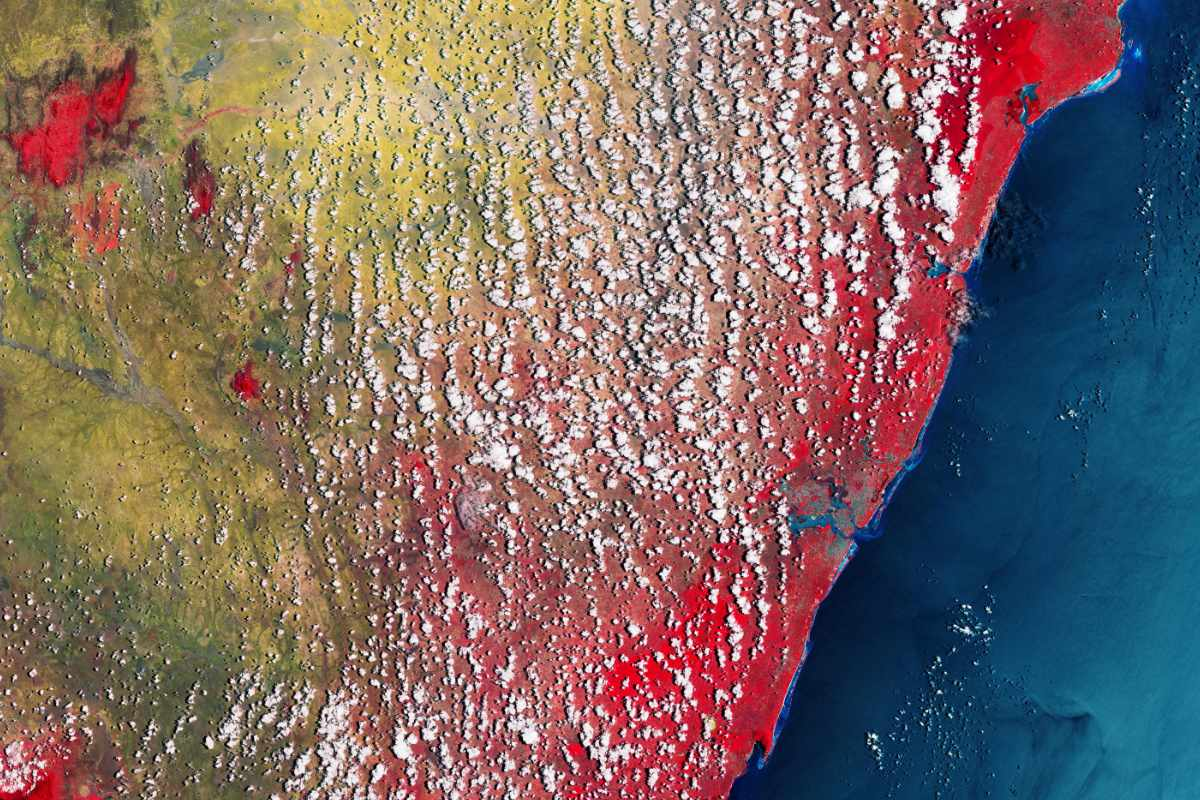
\includegraphics[width=\linewidth]{figures/Earth_from_Space_Southeast_Kenya}
    \caption{Southeast Kenya}
    \label{fig:sentinel_kenya}
  \end{subfigure}
  \hfill
  \begin{subfigure}{.32\linewidth}
    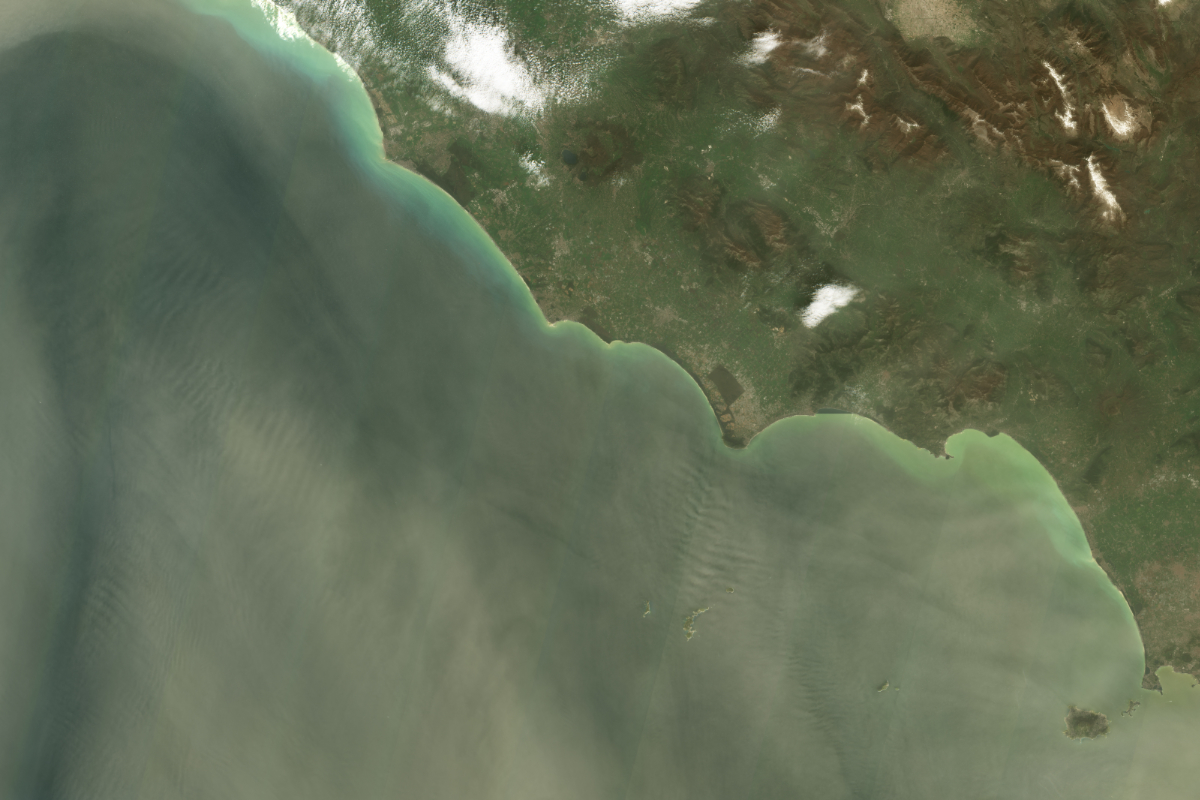
\includegraphics[width=\linewidth]{figures/Saharan_dust_plume}
    \caption{Sahara dust}
    \label{fig:sentinel_sahara}
  \end{subfigure}
  \hfill
  \begin{subfigure}{.32\linewidth}
    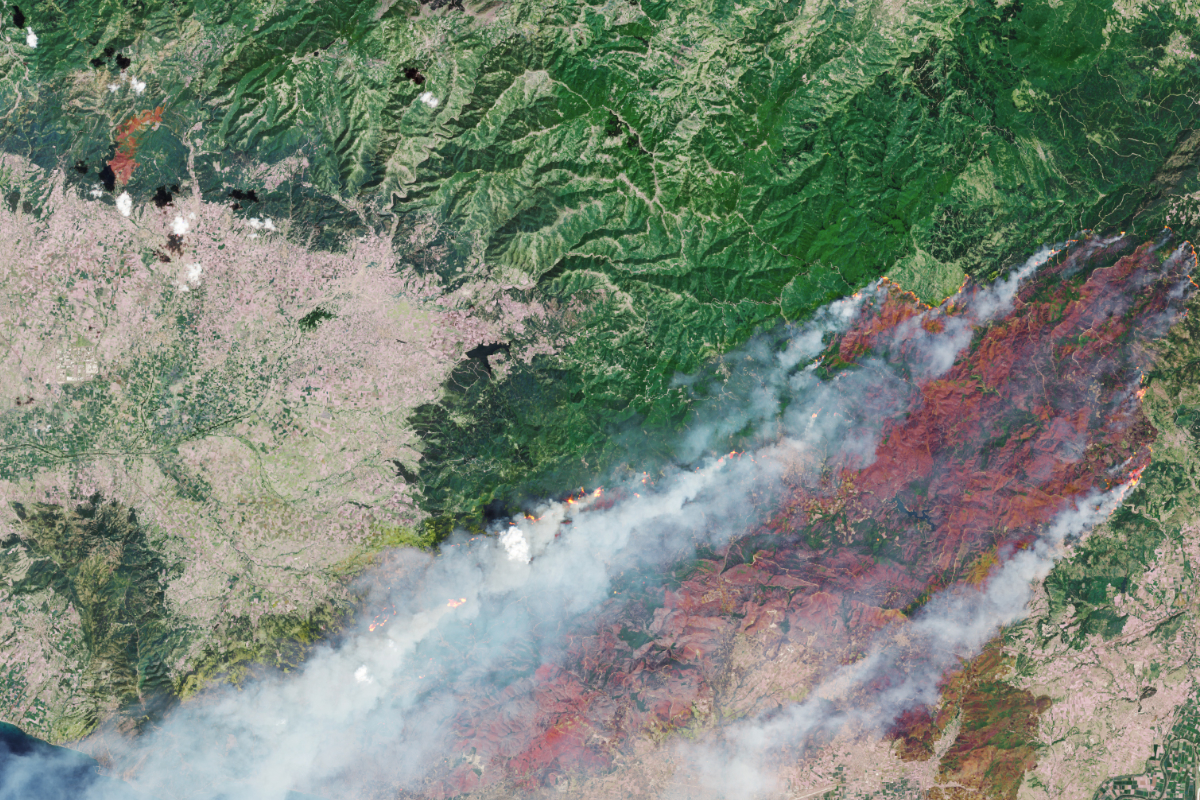
\includegraphics[width=\linewidth]{figures/Wildfires_continue_to_rage_in_Greece}
    \caption{Wildfires in Greece}
    \label{fig:sentinel_greece}
  \end{subfigure}

  \caption{Example images from the \sentinelii mission. (Credit: processed by ESA, CC BY-SA 3.0 IGO)}
  \label{fig:sentinelii}
\end{figure*}

\begin{table}
  \caption{\sentinelii Spectrum Bands}
  \label{tab:sentinel_bands}

  \centering
  \begin{tabular}{llcc}
    \toprule
    Band & Measurement & Central wavelength & Resolution \\
    \midrule
    1 & Coastal aerosol & 443 nm & 60 m \\
    2 & Blue & 490 nm & 10 m \\
    3 & Green & 560 nm & 10 m \\
    4 & Red & 665 nm & 10 m \\
    5 & Vegetation red edge & 705 nm & 20 m \\
    6 & Vegetation red edge & 740 nm & 20 m \\
    7 & Vegetation red edge & 783 nm & 20 m \\
    8 & Near infrared & 842 nm & 10 m \\
    8A & Narrow near infrared & 865 nm & 20 m \\
    9 & Water vapour & 940 nm & 60 m \\
    10 & Short wave infrared: cirrus & 1375 nm & 60 m \\
    11 & Short wave infrared & 1610 nm & 20 m \\
    12 & Short wave infrared & 2190 nm & 20 m \\
    \bottomrule
  \end{tabular}
  
\end{table}

With recent advances in space and image sensing technologies, Earth observation using small satellites has gained more and more attention over the past years.
As an example use case for the methods we propose in this paper, we briefly introduce ESA's \sentinelii mission.
We also use a subset of the mission's dataset for our evaluation.
Moreover, we give an overview of how neuronal networks are used onboard satellites for image processing.

\sentinelii \cite{sentinel2} is a set of missions operated by the \ac{esa} as part of the Copernicus program using \ac{leo} satellites.
The first satellites were launched in 2015, with more launches following in 2017 and 2024.
The missions comprise two satellites, which orbit the Earth such that each spot on the surface is revisited approximately every five days.
With their sensors, they cover a strip of land that is 290 km wide with each pass.
In addition to visible light sensors, the satellites are equipped with sensors that cover additional frequencies, such as infrared \cite{sentinel-2-user-handbook}, which allow to capture land use and vegetation (cf. \Cref{tab:sentinel_bands}).
Moreover, the sensors feature relatively high optical resolutions between 10 and 60 meters.

% https://www.esa.int/ESA_Multimedia/Images/2024/03/Earth_from_Space_Southeast_Kenya
% https://www.esa.int/ESA_Multimedia/Images/2024/04/Saharan_dust_plume
% https://www.esa.int/ESA_Multimedia/Images/2023/08/Wildfires_continue_to_rage_in_Greece

\Cref{fig:sentinelii} shows three example use cases for Earth observation images taken from \ac{esa}'s homepage.
The first (\Cref{fig:sentinel_kenya}) is a false-color image of southeast Kenya, which was generated by overlaying \sentinelii's near-infrared channel onto the visual spectrum.
The bright red colors indicate higher plant density and health, as alive plants reflect near-infrared light.
Thereby, the dense vegetation in the coastal regions can easily be distinguished from the hinterland regions.
\Cref{fig:sentinel_sahara} shows a dust storm originating from the Sahara desert.
\sentinelii provides valuable insights for air pollution monitoring, and due to the short revisit time, storms can be monitored as they develop.
Finally, \Cref{fig:sentinel_greece} shows wildfires in Greece in 2023.
For the visualization, the shortwave infrared spectrum was merged with the visible light spectrum, showing the fire front.
Dark brown areas show the burned area.
Thereby, these images provided valuable insights for civil protection authorities.
By using more efficient and more robust image compression and transmission using \ac{jscc}, sensor data in small satellite missions can be transmitted and used faster, allowing even more rapid responses.

%%% TODO rephrase -v

Since the small size of satellites limits their energy budget, it is necessary to consider energy constraints when deploying neural networks onboard of satellites.
In addressing the system's deployability and energy consumption, we turn to several key studies and missions.

The detection of cargo ships on the ocean from satellite imagery has been tested using an Nvidia TX2 SoC, which not only fits within CubeSat limitations but also sustains a total power envelope of 7.5\,W, making it compatible with small satellite missions \cite{8556744}.
The Intel Movidius Myriad 2 and STM32 Microcontroller, both low-power processors, have successfully executed star identification tasks using neural networks with a power usage of 0.89--1.08\,W for Myriad and 1.15--1.2\,W for STM32 \cite{s20216250}.
On the International Space Station (ISS), deep learning models were evaluated on the Qualcomm Snapdragon 855 and Intel Movidius Myriad X processors, further underlining the feasibility of running a neural network onboard of satellites \cite{9884906}.
A variety of models were tested that were trained on images from Earth and Mars. In particular, rather large standard ML models, such as VGG19 \cite{DBLP:journals/corr/SimonyanZ14a} and ResNet50 \cite{7780459}, were used. 
Moreover, the practical deployment of ML models onboard small satellites was tested in the $\Phi$-Sat mission via the use of Intel Movidius Myriad 2 for onboard cloud detection \cite{9600851}.


\section{Our approach}
\label{sec:our_approach}

\subsection{Overview}

communication model from old paper, fig 2

\subsection{Joint Source and Channel Coding using Neural Networks}

\subsection{Channel Model for LEO Satellites}

\subsection{Attention Modules}

\subsection{Link Budget Analysis}
Identisch zu LCN23

\section{Evaluation}
\label{sec:evaluation}

\section{Conclusion}
\label{sec:conclusion}

\bibliographystyle{IEEEtran}
\bibliography{references}

\end{document}
